\documentclass[a4paper,10pt]{report}
\usepackage[utf8]{inputenc}
\usepackage{listings}
\usepackage[T1]{fontenc}
\usepackage{graphicx}
\usepackage{float}
\usepackage{caption}
% Title Page
\title{Rapport CPA}
\author{Memmi Sacha \\ Shokoufeh}


\begin{document}
\maketitle

\clearpage
\chapter{Préambule}
Les tests que nous avons effectués ont été fait sur une machine possédant 16 Go de RAM ainsi qu'un processeur cadencé à 3.8 Ghz et muni de 12 cores.
\\
Nous avons pu effectuer, au cours de nos recherches, plusieurs implémentations différentes (utilisant différentes structures) dans le but d'optimiser au maximum nos temps d'exécutions. 
\newline 

\chapter{Présentation de nos structures de données}
Nous avons utilisé deux structures de données afin de stocker nos graph en mémoire.
\\
Il y a d'une part adjmatrix qui contient une matrice d'incidence. Elle est pratique car elle est assez intuitive à utiliser. Cependant, dès que le graph que nous utilisons est grand est qu'il n'est pas fortement connexe, cette structure doit être dépréciée au profit de la seconde structure de donneés.
\\
La seconde structure de donnée est la structure adjlist. Cette structure contient un tableau qui indique les degrés cumulés de chaque noeud. 
\\
Chaque extrémité d'une arête peut être retrouvée à l'aide de la matrice adj et du tableau des degrés précedemment introduit.
\\
Les deux structures possèdent deux attributs qui sont, e et n, qui donnent respectivement le nombre d'arête de notre graph ainsi que le nombre de noeuds.
\chapter{Construction et stockage de nos données}
\section{Calcul de la taille du graph}
La fonction readEdgeList nous permet de mettre en mémoire notre graph depuis un fichier stocké. 
\\
Le nombre de noeuds est déjà un attribut de notre structure de données. 
\\Par conséquent, nous n'avons pas besoin de le recalculer, il est fait en même temps que la mise en mémoire de notre graph.

Ci dessous, un tableau donnant le nombre d'arêtes et de noeuds pour différents sets de données ainsi que leur temps d'exécution:
\\

\begin{center}
    \begin{tabular}{|l|c|c|c|}
    \hline
     & nodes & edges & Execution time \\ \hline
     Email & 1005 & 25571 & 0s \\
     Amazon & 548 552 & 925775 & 0s\\
     liveJournal & 4 036 538 & 34 681 046 & 20s\\
     orkut & - & - & non calculé \\
     friendster & - & - & non calculé\\
     \hline
    \end{tabular}
\end{center}
Nous pouvons constater avec le tableau ci-dessus, que dès lors que le graph grandit il devient plus délicat de le mettre en mémoire. \\ 
D'où l'absence de certain résultats.
\\
\section{Nettoyage de nos données}
Afin de nettoyer nos données nous avons utilisé la commande linux suivante :
\begin{lstlisting}
 awk '{if ($1<$2) print $1" "$2;else if ($2<$1) print $2" "$1}' net.txt | sort -n -k1,2 -u > net2.txt
\end{lstlisting}
Celle-ci, permet qu'un noeud ne soit relié qu'à un sommet plus grand que lui dans notre fichier. 
\\
Ainsi, les arêtes ne seront prises en compte qu'une fois. 
\\ 
De plus, cette ligne de commande permet de trier suivant l'extrémité de départ d'un edge puis suivant l'extrémité terminale et supprime les doublons.
\\
\section{Les trois différentes datastructures}
Comme nous le disions dans le préambule, nous préférons travailer avec la structure de données adjacency array plutôt que adjancy matrix. 
\\
\newline
En effet, adjacency matrix stock toutes les arêtes possibles (même celles qui n'existent pas), c'est un gâchis d'espace mémoire dans le cas où notre graph est peu dense et que nous n'avons pas besoin de le modifier.
\\
Nous avons pu expérimenter l'importance de la scalabilité de notre structure de données tout au long de nos recherches.
\\
\newline
Nous permettant ainsi, de remarquer le manque de scalabilité de la structure de données adjacency matrix.
\\
\section{Breadth First Search}
\subsection{Structure de données utilisée}
La structure que nous avons utilisé est l'adjacency array car nous n'avions pas besoin de faire des changements dans notre graph.
\\
Nous avons créée une fifo pour visiter tous les noeuds du graph connexe. 
\subsection{Analyse théorique de la complexité temporelle}
La complexité temporelle théorique est O(\textbf{S+A}). Nous parcourons toutes les arêtes ainsi que tous les noeuds

\section{Diamètre}
\subsection{Structure de données utilisée et sous-structure}
Pour déterminer le diamètre de notre graph, nous avons tout d'abord déterminer la taille de ainsi que les noeuds appartenant à la composante connexe la plus grande.
\\
Nous effectuons NDIAMETER fois la boucle suivante 
\\
Ensuite, nous avons déterminé la distance maximale venant d'un noeud aléatoire de cette composante connexe.
\\
Nous prenons le maximum des valeurs retournées dans notre boucle.
\\
Nous avons donc pris le maximum des distances maximales de NDIAMETER tirés aléatoirement parmis ceux nons visités.
\\
\subsection{Analyse de la complexité théorique}
Ici, ce qui sera le plus coûteux dans notre algorithme sera de repérer la composante connexe maximale. 
\\
\newline
En effet, nous allons devoir faire un bfs sur chaque composante connexe.
\\
Nous aurons dans le pire des cas, une complexité en O(\textbf{U * L*log(L)}).
\newline
U étant le nombre de composantes connexes et L le nombre moyen de noeuds d'une composante connexe.
\subsection{Analyse expérimentale}
Nous avons pu obtenir les temps d'exécution suivants pour un nombre de noeuds NDIAMETER fixé à 100
\begin{center}
    \begin{tabular}{|l|c|}
    \hline
     Set de données & temps d'exécution\\ \hline
     Email & 1s\\ 
     Amazon & 55s\\ 
     Orkut & 4m52s \\
     Live Journal & 3\\ 
     Friendster & 3\\ 
     \hline
    \end{tabular}
\end{center}
Pour ce qui concerne les résultats des diamètres, vous trouverez ci-dessous les résultat pour chaque jeu de données :
\newline
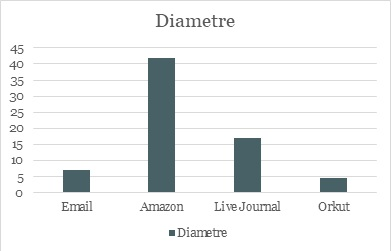
\includegraphics[scale=0.9]{./Datas/diagrammeDiametres.jpg}
\section{Détection de triangles}
\subsection{Structure utilisée}
Pour la détection de triangles, nous avons utilisé la structure de données adjacency array car celle-ci convenait le mieux à notre problème.
\\
\subsection{Analyse théorique de la complexité temporelle}
Dans le pire des cas nous effectuons $n^{3}$ comparaisons si tous les noeuds de notre graph sont connectés.
\\
Autrement dit si notre graph forme une unique clique. Ce qui est un cas très rare. 
\\
En général, nous travaillons sur des graphes moyennement connexe. 
\\
Ce qui nous permet d'obtenir une complexité moyenne bien meilleure ainsi que des temps d'exécution tout à fait intéressant comme nous le verrons dans la section consacrée à l'analyse expérimentale.
\\
\newline
En moyenne, nous aurons une complexité en O(\textbf{$S*L^2$}). 
\\
Avec S le nombre de noeuds et L le nombre moyen de voisins d'un noeud.
\clearpage
\subsection{Analyse expérimentale}
Ci-dessous les résultats obtenus.
\newline
\begin{center}
    \begin{tabular}{|l|c|c|}
    \hline
     Set de données & nombre de triangles détectés& temps d'exécution\\ \hline
     Email & 104 333& 0s\\ 
     Amazon &667 129& 1s\\ 
     Orkut & 627584181& 1h35m38 \\
     Live Journal &177820130 & 4m53s\\ 
     Friendster &non calculable & non calculable\\ 
     \hline
    \end{tabular}
\end{center}
Ci-dessous les résultats de transitivity ratio obtenus:
\\
\begin{center}
    \begin{tabular}{|l|c|c|}
    \hline
     Set de données & transitivity ratio & temps d'exécution\\ \hline
     Email & 0.348518& 0s\\ 
     Amazon &0.314602& 1s\\ 
     Orkut & 627584181& 1h35m38 \\
     Live Journal &0.147386 & 4m22s\\ 
     Friendster &non calculable & non calculable\\ 
     \hline
    \end{tabular}
\end{center}
\chapter{Détection de communautés dans un graph non orienté}
\section{Génération de graph jouet}
Pour la génération d'un graph, nous prenons en argument un nombre de noeuds un nombre de clusters, un p et un q.
\\
Nous effectuons une séparation simple de nos noeuds en clusters en fonction du nombre de clusters donnés en argument.
\\
Un noeud est relié à un autre noeud du même cluster avec une probabilité p.
\\
Un noeud est relié à un autre noeud d'un cluster différent avec une probabilité q.
\newline
\newline
Lorsque nous augmentons p nous augmentons la connexité au sein d'une même communauté.
\\
À contrario, augmenter q rend la discrimination de communautés plus difficile car il rend les communauté du graph nouvellement créé moins facilement identifiable.
\section{label propagation}
Nous avons effectué une implémentation de l'algorithme de label propagation qui attribue à un sommet le label le plus fréquent dans ses voisins.
\\
Pour ce faire, nous avons utilisé la structure adjmatrix car cela nous semblait plus simple et que nous travaillions sur des graphes jouets plus modestes.
\subsection{Analyse de la complexité théorique}
La fonction highest\_density fait dans le pire des cas 1 fois S comparaisons plus 3 fois S comparaisons pour la deuxième boucle. 
\\
Nous conservons une complexité linéaire O(S).
\\
Le core de label\_propagation est une boucle qui itére sur tous les sommets et leur applique highest\_density.
\\
Par conséquent nous avons une complexité en O($S*S$).
\subsection{Analyse expérimentale / Simple Benchmark}
Nous obtenons les résultats suivants:
\\
Les tests ont été effectués avec un p fixé à 0.5. C'est à dire que un noeud a 50 pourcents de chances d'être connecté à un noeud du même cluster. 
Nous fixons le nombre de clusters à 8 et le nombre de noeuds à 400.
\\
Nous obtenons les résultats suivants :\\

 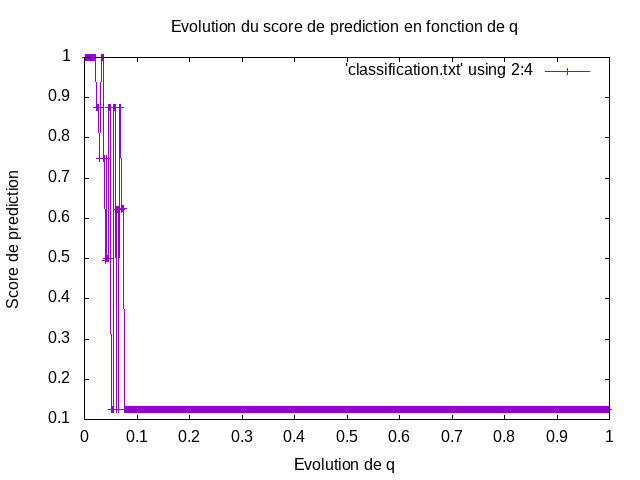
\includegraphics[scale=0.6]{Datas/classificationp05scorelabelpropagation.png}
Nous constatons que notre score de prédiction diminue très rapidement lorsque q augmente. 
\\
Ce qui est logique, car plus q augmente plus nous diminuons notre capacité de distinction entre les communautés.
\\
Pour q = 0.036
\\
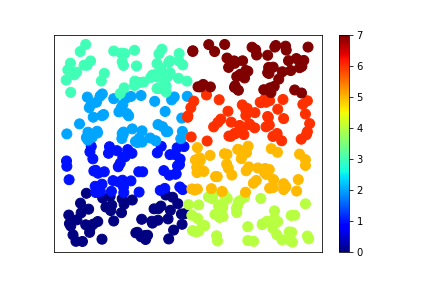
\includegraphics[scale=0.6]{Datas/colorLabelPropagation036.png}
\\
Pour q = 0.04
\\
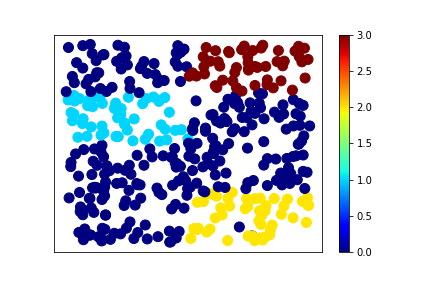
\includegraphics[scale=0.6]{Datas/colorLabelPropagation040.png}
Nous constatons ici qu'il commence à y avoir des chevauchements entre les vraies communautés et les communautés détectées.
\\
Nous avons vérifié, notre algorithme renvoie des résultats corrects lorsque le graph est extrêmement grand.
\section{Algorithme de Jaccard}
Nous avons choisi d'implémenter un label propagation basé sur l'indice de Jaccard. 
\\
\newline
Pour rappel, l'indice de Jaccard permet de calculer la similarité entre les voisins de deux noeuds distincts.
\\
sa formule est donnée par :
\\
\begin{center}
$S(v_i,v_j) = \frac{ T_{v_i} \cap T_{v_j} }{T_{v_i} \cup T_{v_j}}$
\end{center}
Dans notre algrithme, nous utilisons deux fois l'indice de Jaccard. 
\\
Une fois pour déterminer la similarité entre deux noeuds dans le but trier nos noeuds dans l'ordre de similarité du plus grand vers le plus petit.
\newline
La seconde fois où nous utilisons l'indice de Jaccard c'est pour connaître la similarité entre un noeud et une communauté.
\newline
Ce calcul constitue la partie la plus fondamentale de notre algorithme.
\clearpage
\subsection{Analyse expérimentale}
Nous avons conservé le même procédé afin de comparer l'efficacité de nos différents algorithmes.
\\
Nous avons donc toujours un p fixé à .5, un nombre de noeuds fixé à 400 ainsi qu'un nombre de clusters fixé à 8.
Nous obtenons le graph suivant :
\newline
\\
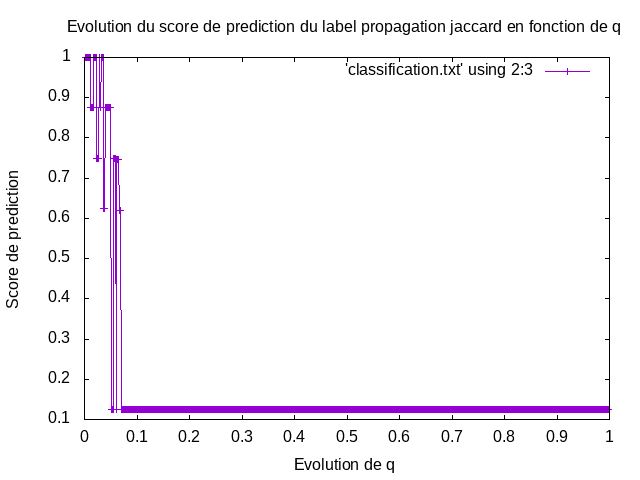
\includegraphics[scale=0.6]{./Datas/classificationp05ScoreJaccard.png}
\\
Nous voyons que notre algorithme donne à peu près les mêmes résultats que le label propagation que nous avons mentionné précedemment.
\\
Cependant, il est tout de même moins stable dans ses résultats.
\section{Louvain personnel}
Nous avons aussi codé un label propagation de Louvain cependant il n'est absolument pas robuste.
\\
Voici les résultats obtenus pour q=.15
\\
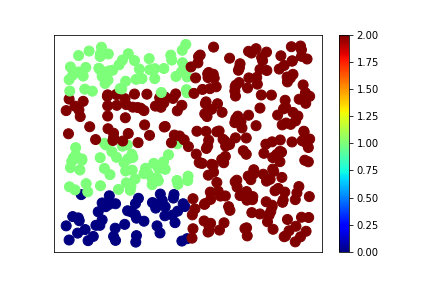
\includegraphics[scale=0.6]{./Datas/colorLouvain015.png}
\section{Comparaisons des trois algorithmes}
Nous superposons les graphes de tous nos résultats:
\\
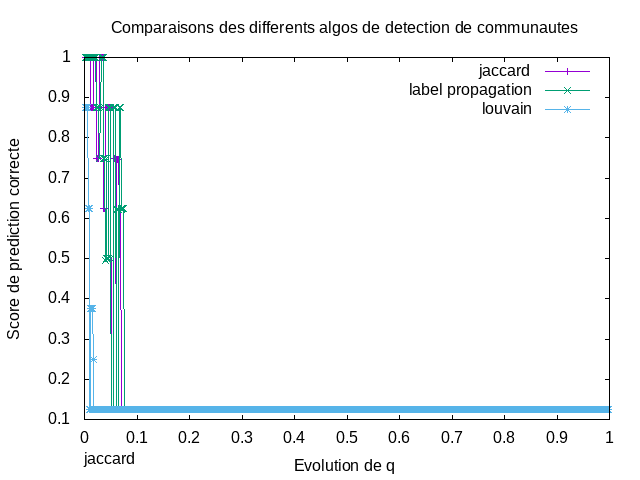
\includegraphics[scale=0.6]{./Datas/compareDetectionsAlgos.png}
Nous remarquons que nos deux algorithmes précedents étaient bien plus efficace que le Louvain que nous avons implémenté.
\\
\section{Experimental Evaluation du louvain fourni}
\subsection{Analyse temporelle}
Tout d'abord, selon nos analyses théoriques précédentes, nous pensons que la complexité temporelle est à peu près égale à O($S^2$).
\\
Regardons si les analyses expérimentales que nous avons mener nous permet de vérifier cette assertion.
\\
Ci-dessous le graph de l'évolution des temps d'exécutions en fonction du nombre de noeuds présents dans notre graphe.
\\
Nous avons fixé p à 0.5, q à 0.4 et le nombre de clusters à 8 pour la génération de nos graph.
\\
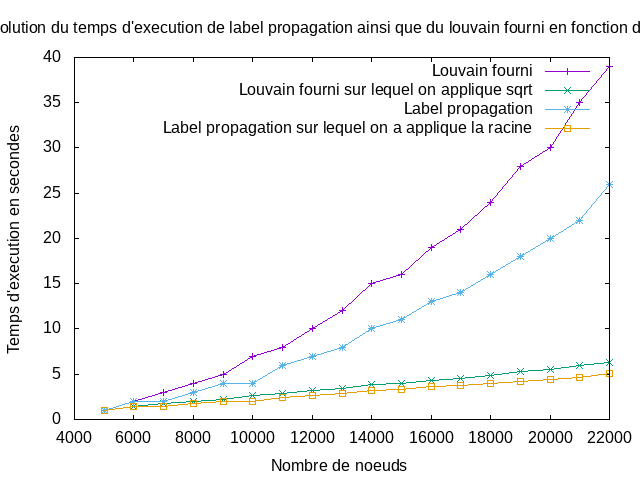
\includegraphics[scale=0.6]{./Datas/graphTempsExecutionLabelLouvain.png}
\\
\newline
En violet, nous avons le graph des temps d'exécution du Louvain fourni.
\\
En bleu, nous avons les temps d'exécution du Label Propagation.
\\
\\
Tout d'abord, nous constatons que notre algorithme est légèrement plus rapide que celui fourni.
\\
Comme nous le disions précédemment, nous pouvons voir que les courbes ont une forme de fonctions carré.
Pour vérifier cela, nous avons aussi afficher en vert et jaune les courbes respectivement de Louvain et du Label propagation sur lesquelles on a appliqué la fonction racine carré. 
\\
Nous constatons que l'application de cette fonction a linéarisée nos courbes. 
\\
Notre intuition était donc correcte.
\\
\subsection{Analyse accuracy}
Les résultats que nous avons pu obtenir ont été obtenu pour :\\
-5000 noeuds\\
-p = 0.5\\
-q varie de 0.1 à 1\\
-10 clusters\\
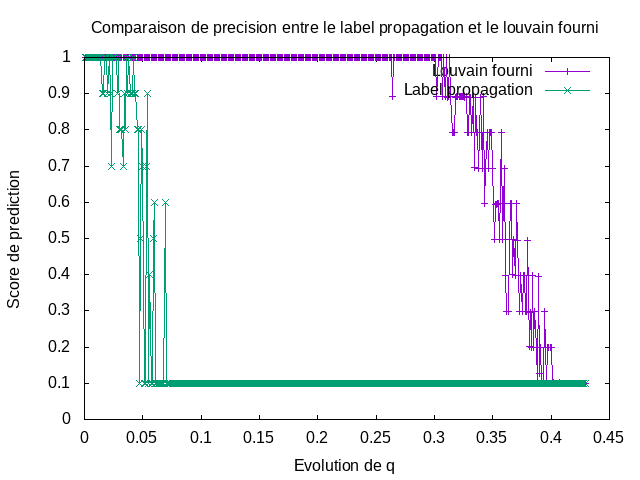
\includegraphics[scale=0.5]{./Datas/evalScoreLabelLouvain.png}
\\
Nous constatons sans surprise que la précision du programme fourni est bien plus robuste à l'augmentation de q par rapport à celle du label propagation que nous avons codé.\\
Il faut attendre que le ratio $\frac{p}{q}$ soit proche de 1 pour que la précision du programme fourni commence à réduire de manière significative.
\\
\subsection{Comparaisons des deux algorithmes}
Pour temperer l'utilité de notre algorithme, il convient de rappeler que q est la probabilité qu'un noeud soit relier à un noeud d'un autre cluster.
\\
Ainsi, plus le graph contient de noeuds plus nos noeuds seront reliés aux noeuds d'autres clusters.
\\
Habituellement, q est très faible.
\\
En général, on a une connexité très basse entre noeuds de clusters différents. Par conséquent, notre algorithme peut s'avérer tout à fait pertinent. 
\\
D'autant plus qu'il est plus rapide que celui du Louvain fourni.
\\
Pour conclure, lorsque l'on sait qu'il n'y a pas une grande connexité entre les noeuds de clusters différents, il est préférable d'utiliser notre algorithme.
\\
Si l'on cherche la précision, il est au contraire préférable d'utiliser le programme fourni dans l'exercice.
\\
\chapter{Page Rank}
\section{Préambule}
Le but de cet algorithme est de trouver la matrice stationnaire vers laquelle converge un graph.
\\
La somme de tous éléments du vecteur que nous renvoie notre algorithme fait 1.
\\
L'algorithme nous renvoie la probabilité de se trouver en chaquenoeud après une infinité d'itérations.
\\
Il permet de déterminer le vecteur propre de la matrice représentant notre graphe.
\\
Pour rappel, le vecteur propre X d'une matrice A est tel que:\\
$AX = \lambda X$
\\
Il s'agit d'algorithmes primordiaux dans le fonctionnement des moteur de recherches.
\section{Exercice 1}
Pour arriver à converger, 11 itérations sont suffisantes.
\\
voici les 5 pages avec les hauts ranks et 5 pages avec les bas rank
\begin{table}[ht]
\caption{5 page avec plus bas score}
\centering
\begin{tabular}{|c c c c|}
\hline\hline
Number & PageScore & PageNumber & PageName \\[0.5ex]
\hline
1 & 0.000004 & 691802 & Ethics \\
2 & 0.000004 & 691565 & Humor \\
3 & 0.000004 & 691566 & Geometry  \\
4 & 0.000004 & 690803 & Calculus \\
5 & 0.000004 & 690637 & Algebra \\
\hline
\end{tabular}
\label {table:nonlin}
\end{table}

\begin{table}[ht]
\caption{5 page avec haut bas score}
\centering
\begin{tabular}{|c c c c|}
\hline\hline
Number & PageScore & PageNumber & PageName \\[0.5ex]
\hline
1 & 0.000100 & 12541226 & Maps of the Caliphate \\
2 & 0.000085 & 6801297 & Old maps of Austria-Hungary \\
3 & 0.000077 & 4392379 & Napoleonic Wars  \\
4 & 0.000076 & 5851224 & People from Richmond, Virginia \\
5 & 0.000070 & 690451 & World War II \\
\hline
\end{tabular}
\end{table}

\section{Correlations}
Nous avons exécuté l’algorithme pour donner ce qui est dans catHier\_allDirLinks avec régression liner pour ces données.\\
Nous avons obtenus les graphes suivants:
\\
Indegrees:
\\
\begin{figure}[H]
  \caption{x = PageRank with  = 0.15, y = in-degree.}
  \centering
    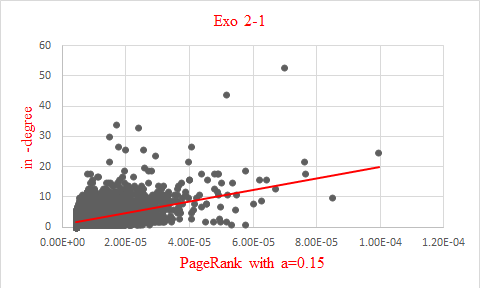
\includegraphics{./Datas/pageRank/pageRankAlpha015Indegree.png}    
\end{figure}
Outdegrees
\begin{figure}[H]
 \centering
  \caption{x = PageRank with  = 0.15, y = out-degree}
    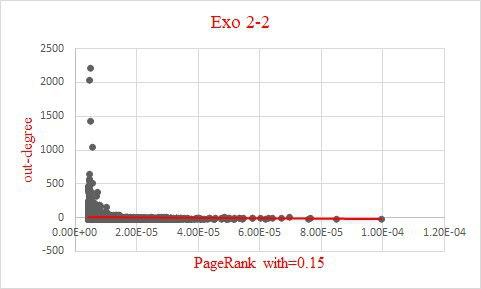
\includegraphics{./Datas/pageRank/pageRankAlpha015Outdegree.jpg}
\end{figure}
$\alpha = 0.15, \alpha = 0.1$
\begin{figure}[H]
  \caption{x = PageRank with  = 0.15, y = PageRank with  = 0.1}
  \centering
    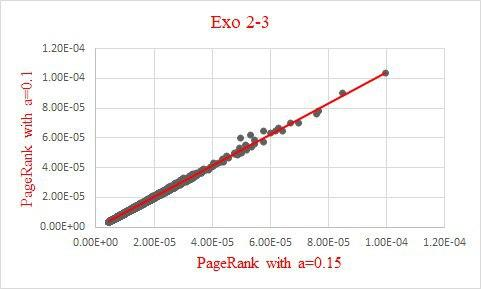
\includegraphics{./Datas/pageRank/pageRankAlpha015PageRankAlpha01.jpg}
\end{figure}
$\alpha = 0.15,\alpha= 0.2$
\begin{figure}[H]
  \caption{x = PageRank with  = 0.15, y = PageRank with  = 0.2}
  \centering
    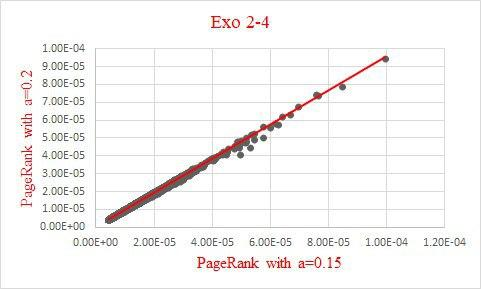
\includegraphics{./Datas/pageRank/pageRankAlpha015Alpha02.jpg}
\end{figure}
$\alpha =0.15,\alpha=0.5$
\begin{figure}[H]
  \caption{x = PageRank with  = 0.15, y = PageRank with  = 0.5}
  \centering
    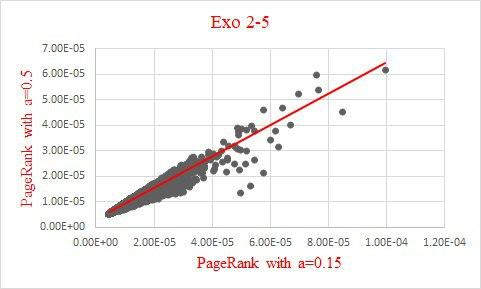
\includegraphics{./Datas/pageRank/pageRankAlpha015Alpha05.jpg}
\end{figure}
$\alpha =0.15,\alpha=0.9$
\begin{figure}[H]
  \caption{x = PageRank with  = 0.15, y = PageRank with  = 0.9}
  \centering
    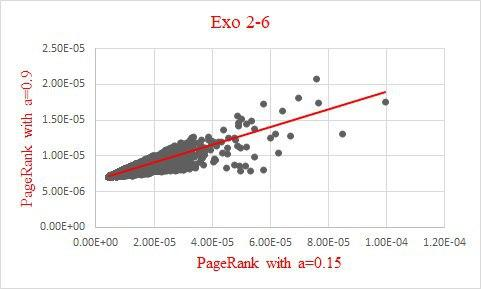
\includegraphics{./Datas/pageRank/pageRankAlpha015Alpha09.jpg}
\end{figure}
$\alpha =0.15,\alpha=0.9$ log scale
\begin{figure}[H]
  \caption{x = PageRank with  = 0.15, y = PageRank with  = 0.9 with not linear regression }
  \centering
    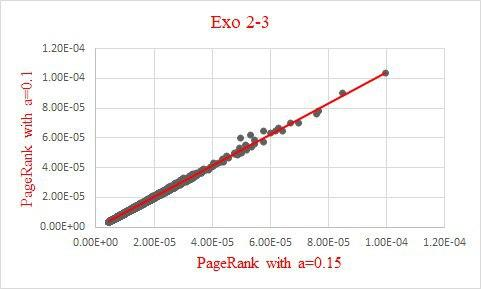
\includegraphics{./Datas/pageRank/pageRankAlpha015PageRankAlpha01.jpg}
\end{figure}
1)Il est préférable d'utliser l'échelle logarithmique car elle permet de linéairser grandement la distribution.\\
2)En regardant la corrélation sur le dernier graph nous constatons qu'il existe une forte corrélation entre x et y. En effet, lorsque nous augmentons le $\alpha$ du y nous constatons que les valeurs de score de régression s'éloigne de la droite de régression.
\\
\chapter{Densest subgraph}
\section{Préambule}
Comme chacun sait, l'analyse de la densité d'un graph est un outil précieux de data mining.
Il permet, à partir d'un graph qui peut paraître opaque de détecter classer les différents noeuds de notre graph un peu à la manière de la détection de communautés. 
\\
Comme pour la détection de communauté, l'algorithme repose sur la connexité de nos noeuds.
\\
Cependant avec la décomposition kcore, nous raisonnons de l'extérieur du graph vers l'intérieur du graph. Il y a une notion d'imbrication dedans.
\\
Dans ces parties (EXO1 etEXO3) nous avons calculé le core value et score de chaque nodes et nous avons sorte les nodes en base de core value et score et pour chaque ces parties nous avons trouvé le average degrés densité pour chaque sousgraph (n premiere sougraph) et rendre le maximum entre eux et les nombres des nodes de se sousgraphe. pour trouver les score des nodes nous avons teste pour different iteration. 
nous avons aussi calcule le degree densite plus haute et les comparer.
\\
\section{Analyse de la densité}
Pour commencer nous avons créé nos algorithme de core decomposition afin de pouvoir faire une analyse des densités demandés.
\\
Notre algorithme se base sur une boucle qui, au début, prend le premier sous graph pris dans l'ordre donné par core decomposition.\\
Puis le premier et le second élément et ainsi de suite.
\\
\\
À l'issue de l'exécution de cet algorithme, nous avons:\\
\indent -core qui indique le degré du noeud.\\
\indent -order qui indique l'ordre de chaque noeud
        \\
        \\
Comme dit plus haut, l'algorithme core decomposition nous a permis de calculer la densité moyenne des degrés dans notre graph complet.
\\
Grâce à cela, nous avons pu voir un peu plus clair dans notre jeu de données.
\clearpage
Voici les résultats de k-core decomposition ainsi que les résultats de average degree density le max average degree density ainsi que le edge density.
\begin{table}[ht]
\caption{k-core decomposition}
\centering
\begin{tabular}{|c c c c c|}
\hline\hline
name & Average degree density graph complet & max Average Degree Density(i) & Edge density(ii) & Size of the densest core ordering prefix(iii) \\[0.5ex]
\hline

Email & 50.88 & 30.5 & 2.1 & 9 \\
Amazon & 3.375 & 13.5 & 0.94 & 8 \\
LiveJournal & 17.83 & 45.7 & 2.7 & 15  \\

\hline
\end{tabular}
\label {table:nonlin}
\end{table}

\section{Exercice 2}

\section{Exercice 3}

\begin{table}[ht]
\caption{densest subgraph avec t=10}
\centering
\begin{tabular}{|c c c c c|}
\hline\hline
name & max Average Degree Density(i)&Edge density(ii)&Size of the densest core ordering prefix(iii) & time of calcul \\[0.5ex]
\hline

Email & 15.4 & 1.07 & 8 & 1s \\
Amazon & 1.14 & 0.095 & 7 & 49s \\
LiveJournal & &  &  &   \\

\hline
\end{tabular}
\label {table:nonlin}
\end{table}

\begin{table}[ht]
\caption{densest subgraph avec t=100}
\centering
\begin{tabular}{|c c c c c|}
\hline\hline
name & max Average Degree Density(i)&Edge density(ii)&Size of the densest core ordering prefix(iii) & time of calcul \\[0.5ex]
\hline

Email & 18.28 & 1.5 & 7 & 1s \\
Amazon & 2.66 & 0.666 & 3 & 44s \\
LiveJournal & &  &  &   \\

\hline
\end{tabular}
\label {table:nonlin}
\end{table}

\begin{table}[ht]
\caption{densest subgraph avec t=1000}
\centering
\begin{tabular}{|c c c c c|}
\hline\hline
name & max Average degree Density(i)&Edge density(ii)&Size of the densest core ordering prefix(iii) & time of calcul \\[0.5ex]
\hline

Email & 17.7 & 1.5 & 7 & 2s \\
Amazon & 2.66 & 0.666 & 3 & 58s \\
LiveJournal & &  &  &   \\

\hline
\end{tabular}
\label {table:nonlin}
\end{table}

\begin{table}[ht]
\caption{max average density for graphs}
\centering
\begin{tabular}{|c c |}
\hline
Email & 47 \\
Amazon & 5 \\
LiveJournal & 124  \\
\hline
\end{tabular}
\label {table:nonlin}
\end{table}
\chapter{Conclusion}
Durant toutes nos recherches nous avons pu utiliser différentes structures de données dans le but de répondre à des problématiques très actuelles. 
\\
Nous avons pu étudier des algorithmes permettant de détecter des communautés, de page ranker un graph, ou encore de décomposer un graph en différents cores et de détecter des cliques.
\\
\newline
Pour répondre à toutes ces problématiques, nous avons dû utiliser les structures de données les plus appropriées afin de garder sous contrôle les temps d'exécution ainsi que l'espace mémoire consommée par nos programmes.
\newline
Nous avons pu constater une nouvelle fois que les structures de données les plus appropriées pour répondre à une problématique peuvent fluctuer.
\\
Ainsi, lorsque nous voulons modifier le graph ou qu'un graph est fortement connexe, il est préférable d'utiliser l'adjacency matrix.\\
Alors que lorsque nous travaillons avec des graphes très grands et pas très connexes il est préférable d'utiliser la structure de données adjacency array.
\newline
\\
À une époque où les quantités de données échangées explosent, il peut s'avérer salvateur de bien réflechir aux structures de données mises en jeu lors de l'utilisation d'un programme.

\end{document}          
